%
% Complete documentation on the extended LaTeX markup used for Insight
% documentation is available in ``Documenting Insight'', which is part
% of the standard documentation for Insight.  It may be found online
% at:
%
%     http://www.itk.org/

\documentclass{InsightArticle}


%%%%%%%%%%%%%%%%%%%%%%%%%%%%%%%%%%%%%%%%%%%%%%%%%%%%%%%%%%%%%%%%%%
%
%  hyperref should be the last package to be loaded.
%
%%%%%%%%%%%%%%%%%%%%%%%%%%%%%%%%%%%%%%%%%%%%%%%%%%%%%%%%%%%%%%%%%%
\usepackage[dvips,
bookmarks,
bookmarksopen,
backref,
colorlinks,linkcolor={blue},citecolor={blue},urlcolor={blue},
]{hyperref}
% to be able to use options in graphics
\usepackage{graphicx}
% for pseudo code
\usepackage{listings}
% subfigures
\usepackage{subfigure}


%  This is a template for Papers to the Insight Journal. 
%  It is comparable to a technical report format.

% The title should be descriptive enough for people to be able to find
% the relevant document. 
\title{Parallel algorithms for erosion and dilation of label images.}

\newcommand{\IJhandlerIDnumber}{999}

% Increment the release number whenever significant changes are made.
% The author and/or editor can define 'significant' however they like.
\release{0.00}

% At minimum, give your name and an email address.  You can include a
% snail-mail address if you like.
\author{Richard Beare{$^1$} {\small and} Paul Jackway{$^2$}}
\authoraddress{Richard.Beare@monash.edu\\Department of Medicine\\Monash University\\Melbourne\\Australia{$^1$}\\CSIRO Mathematics Informatics and Statistics\\Dutton Park\\Queensland\\Australia{$2$}}

\begin{document}

\IJhandlefooter{\IJhandlerIDnumber}

\maketitle

\ifhtml
\chapter*{Front Matter\label{front}}
\fi


\begin{abstract}
\noindent
It is sometimes useful to be able to apply binary morphological
operations, such as erosions and dilations, to labelled images in a
fashion that preserves the labels. This article introduces a
specialised class implementing parallel methods described in
\cite{beare2011parallel} that provide very fast dilations by circles
and spheres of arbitary size.
\end{abstract}

\tableofcontents

\section{Introduction}
The link between Euclidean distance transforms and binary
morphological operations is well known - erosions and dilations by
circles and spheres can be performed by thresholding the distance
transform. Efficient and readily parallelizable distance transform
algorithms can, in turn, be based on erosions and dilations by
parabolic structuring elements. The classes outlined in this article
extend the contact point algorithm used for parabolic erosions and
dilations to facilitate operations on label images. A more complete
discussion is available in \cite{beare2011parallel}. The classes
introduced here are able to separate touching labels during erosion
and split touching labels at the midpoint during dilation.

\section{The classes}
The {\em itk::LabelSetDilateImageFilter} and {\em
  itk::LabelSetErodeImageFilter} implement dilation and erosion of
label images. They share a common parent class. The methods controlling class behaviour are:
\begin{itemize}
\item {\em UseImageSpacing}: Defines whether the radius refers to voxels or world dimensions. Default is false, meaning radius is in voxels.
\item {\em Set/GetRadius}: Set the size of the dilation or erosion. There are versions to set the size in all directions to be the same, corresponding to a circular or spherical structuring element, and independently, corresponding to an ellipsoid structuring element (with axes parallel to image axes).
\end{itemize}

Examples of use are available with the package.

Please note that these are specialised classes which cannot use
arbitrary structuring elements.
\subsection{Notes for label erosion}
The class provided for label erosion {\bf will separate} touching
labels. If this is not the desired behaviour, then implement label
erosion via binary erosion and masking.

\section{Sample results}
Label images occur in many situations. This is an example of a brain
atlas in which different labels represent different anatomical
regions. Examples of 2D processing (operations applied to a single slice of the atlas) are shown in Figure \ref{2d}. Examples of a 3D processing are shown in Figures \ref{fig:3dorig} to \ref{fig:3ddil}.

\begin{figure}[htbp]
\centering
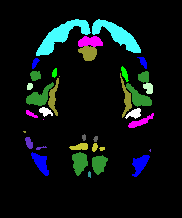
\includegraphics[scale=0.75]{axial_color}
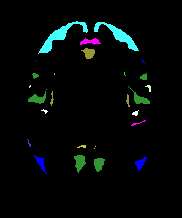
\includegraphics[scale=0.75]{laberode2d_color}
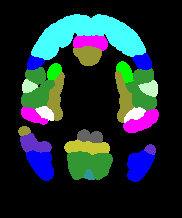
\includegraphics[scale=0.75]{labdilate2d_color}
\caption{Original, eroded and dilated atlases - a single slice with a 2d circular structuring element.\label{fig:2d}}
\end{figure}

\begin{figure}[htbp]
\centering
\includegraphics[scale=0.15]{atlas_orig}
\caption{Axial, sagittal and coronal slices through a labelled brain atlas.\label{fig:3dorig}}
\end{figure}

\begin{figure}[htbp]
\centering
\includegraphics[scale=0.15]{atlas_erode_color}
\caption{Atlas in Figure \ref{fig:3dorig} after applying 3d labelled erosion. \label{fig:3dero}}
\end{figure}

\begin{figure}[htbp]
\centering
\includegraphics[scale=0.15]{atlas_dilate_color}
\caption{Atlas in Figure \ref{fig:3dorig} after applying 3d labelled dilation. \label{fig:3ddil}}
\end{figure}


\section{Alternative approaches to label dilation}
As advised on the ITK mailing list, label dilation can be implemented
via distance transforms and watershed transforms. SimpleITK python code courtesy of Bradely Lowekamp:

\lstset{language=Python}
\begin{lstlisting}
def MultilabelDilation(img, radius=1,kernel=sitk.BinaryDilateImageFilter.Ball):
    distImg = sitk.SignedMaurerDistanceMap(img != 0,
                                           insideIsPositive=False, 
                                           squaredDistance=False, 
                                           useImageSpacing=False)
    dilatImg = sitk.BinaryDilate(img!=0, radius, kernel)
    wsImg = sitk.MorphologicalWatershedFromMarkers(distImg, img)
    return dilatImg*wsImg
\end{lstlisting}

The specialised method should be significantly faster than this approach - perhaps a concientious reviewer can verify?

\bibliographystyle{plain}
\bibliography{local,InsightJournal}
\nocite{ITKSoftwareGuide}

\end{document}

